\chapter{Range Length Evaluations}

This chapter is about finding the minimum range length for \ac{OTA}-\ac{TRP}-measurements. The range length induced measurement error is expected to be dependent of the probe antenna and the measurement distance. For that propose a simulation and a measurement was developed and carried out. Classically \ac{OTA} conformance testing is carried out in the \ac{FF}. In the \ac{mmW} length this hence to some difficulties. To illustrate that, there is an example.

\section{Example: Classical OTA measurement distance}

A \ac{UE} operating at $\SI{28}{\giga\hertz}$ is assumed and shall be tested for the American market. Regarding table \ref{tab:legusa} the maximum frequency to test is $f = \SI{100}{\giga\hertz}$. On the one hand \acp{OEM} wont publish where there antennas are and what their characteristics are. On the other hand \ac{SE} are unintended radiations, so perhaps the radiating element was not meant to be an antenna. So the so called black box approach has to be taken with no pre knowledge of the \ac{DUT}. In worst case configuration it must be assumed that the coherent radiating elements are spread over the howl aperture of the \ac{DUT}. With that assumption a typical smart phone diameter of $D=\SI{15}{\centi\meter}$ is chosen. This leads to a \ac{FF}-distance (refer to equation \ref{eq:ff}) of 

\begin{equation}
r_{\text{FF}} = \frac{2D^2}{\lambda} = \frac{2D^2\cdot f}{c} = \SI{15}{\meter}\,.
\end{equation}

This brings two major problems, first the dynamic range and second the costly measurement environment. The \ac{FSPL} is regarding to formula \ref{eq:fspl}

\begin{equation}
L_{\text{FSPL}} = 20\log_{10}\left(\frac{4\pi r_{\text{FF}} \cdot f}{c}\right)\si{\decibel} = \SI{96}{\decibel}\,.
\end{equation}

With $\SI{15}{\decibel}$ gain from the probe antenna and a noise floor at the \ac{DUT} at $\SI{-23}{\decibelm}$ \ac{EIRP} (to have $\SI{10}{\decibel}$ dynamic range) the resulting power at the probe antenna port would be $P_{\text{Probe Port}} = \SI{-23}{\decibelm}-\SI{96}{\decibel}+\SI{15}{\decibel}=\SI{-104}{\decibelm}$. The \ac{NF} of the complete measurement equipment will be at least $\SI{20}{\decibel}$ including \acp{LNA} and the \ac{VSA} (compare figure \ref{fig:danl}). With that the maximum \ac{RBW} would be 

\begin{equation}
\SI{-174}{\decibelm\per\hertz}+\SI{20}{\decibel}-\left(\SI{-104}{\decibelm}\right)=\SI{-50}{\decibel}\ \Rightarrow\ f_{\text{RBW}}=\SI{100}{\kilo\hertz}\,.
\end{equation}

The required \ac{RBW} is $\SI{1}{\mega\hertz}$, hence to summation of measurement points and lengthy measurements.\\
The cost of \acp{AC} is mainly dependent of the absorber area and the price of the space for the measurement chamber itself. The absorber area is cubically dependent of the range length.
\section{Simulation}

As demonstrated there is the need to find a smaller range length than \ac{FF} distance for ease and efficient measurements. To evaluate the influence of the measurement distance and the probe antenna this simulation was invented and introduced by Benoit Derat and Gerhard Hamberger \cite{mypaper} and is further developed in the framework of this work.

\subsection{Theory}

\begin{figure}[h]
\centering
\def\svgwidth{0.5\textwidth}
\input{Bilder/simPlot.pdf_tex}
\caption{Abstract TRP measurement}
\label{fig:trpmeas}
\end{figure}

For this simulations three spherical surfaces are needed. First the minimal sphere enclosing the \ac{DUT} $S_1$, second the minimal sphere enclosing the probe antenna $S_2$ and third the measurement sphere $\Sigma$ with radius $R$. The origin of the coordinate system is the phase center of the \ac{DUT} ($x$, $y$ and $z$). A sub coordinate system has it's origin in the phase center of the probe and is aligned with it ($u_\phi$, $u_\theta$ and $u_r$). The \ac{EM} emission of the \ac{DUT} is described by the vector fields $E_1$ and $H_1$; the \ac{EM} emission of the probe antenna is analogue to that $E_2$ and $H_2$.\\
The \ac{TRP} is, as described in section \ref{sec:anch}, the cumulated active power flowing through a closed surface enclosing the source. So it is the surface integral over the real part of the Poynting-Vektor \cite{mypaper}. Choosing this surface to be the in figure \ref{fig:trpmeas} depicted surface $S_1$ hence to

\begin{equation}
\text{TRP}=\frac{1}{2}  \oiint_{S_1} \operatorname{Re}\left[E_1	\times H_1^*\right]dS\,.
\end{equation}

Where $dS$ is the vector surface element oriented towards $u_r$. It can be expressed by using the normal vector $n_\text{Sphere}$, pointing radial from the spheres surface leading to the surface 

\begin{equation}
dS = n_\text{Sphere}\sin\left(\theta\right) d\theta d\phi\,.
\end{equation}

With that all spherical integrals can be solved numerically by the quadratures introduced in section \ref{sec:quadrature}. The dot product between the integrand and the normal vector $n_\text{Sphere}$ is projecting the three dimensional integrand on the normal vector and the total length is summed up.\\
Because a real antenna only measures the electric $E$ or the magnetic $H$ component of a \ac{EM} wave in ether horizontal $u_\phi$ or vertical $u_\theta$ polarisation the probe must be evaluated. The measured power of the probe antenna $P_\text{meas}$ in any solid angle $\Omega$ is derivable by the in \cite{book} introduced equations of power transmission

\begin{equation}
P_\text{meas}\left(\Omega\right) = \frac{\big|\oiint_{S_2\left(\Omega\right)}\left(E_1\times H_2 - E_2\times H_1\right)dS\big|^2}{8\oiint_{S_2\left(\Omega\right)}\operatorname{Re}\left[E_2\times H_2^*\right]dS}\,.
\end{equation}

$S_2\left(\Omega\right)$  is the surface enclosing the probe at the position given by the solid angle $\Omega$. The radiated vectorfield of the probe antenna must be known; but the radiating power is irrelevant because the measured power is normalized to it. To derive the \ac{TMP} the measured power must be integrated over the surface $\Sigma$ (compare to figure \ref{fig:trpmeas}) \cite{mypaper}

\begin{equation}
\text{TMP}=\oiint_\Sigma P_\text{meas}\left(\Omega\right)d\Omega = \oiint_\Sigma \frac{\big|\oiint_{S_2\left(\Omega\right)}\left(E_1\times H_2 - E_2\times H_1\right)dS\big|^2}{8\oiint_{S_2\left(\Omega\right)}\operatorname{Re}\left[E_2\times H_2^*\right]dS} d\Omega\,.
\label{eq:trpint}
\end{equation}  

\subsection{Implementation}

For the all quadratures a $\SI{5}{\degree}$ \ac{CSSG} is used. There are three main steps for the implementation of this simulation:

\begin{enumerate}
\item The $E$- and $H$-field of the probe antenna is computed via CST Microwave Studio\texttrademark{} by the integral solver at the $\SI{5}{\degree}$ \ac{CSSG}. If the antenna is more complex and thus unsolvable for the integral solver, the time-domain solver is taken and the antennas characteristics are exported as a \ac{NF}-source which than can be simulated by integral solver. With the integral solver it's possible to compute $E$ and $H$ field components at arbitrary points in the surrounding volume. This needs to be done for horizontal and vertical polarisation.
\item Referring to equation \ref{eq:trpint} a \ac{TMP}-measurement-simulation consists of the outer integral over the measurement sphere $\Sigma$ and the inner integral over the minimum sphere surrounding the probe $S_2$. This means that for every solid angle $\Omega$ the \ac{EM}-field from the \ac{DUT}-antenna on every sphere $S_2$ needs to be computed. The \ac{CSSG} from sphere $S_2$ is always radial aligned, so that the \ac{EM}-field of the probe antenna is valid for every $\Omega$. With $\Delta\phi=\Delta\theta=\SI{5}{\degree}$ this results in
\begin{equation}
N_\text{TMP}=\left(\left(\frac{\SI{180}{\degree}}{\Delta\theta}+1\right)\cdot\frac{\SI{360}{\degree}}{\Delta\phi}\right)^2=2664^2=7,096,896
\end{equation}
measurement points. This is not feasible with the integral solver from CST Microwave Studio\texttrademark{}. Because of that the \ac{NF}-data is fed in to the \ac{FIAFTA}. Occupying the \ac{FIAFTA}, the \ac{EM}-field-calculation at every point in the volume is carried out more efficient.\cite{mypaper} \cite{fiafta}
\item The resulting field data is exported to Matlab\texttrademark{}. There the quadrature of the integral from equation \ref{eq:trpint} is solved and the simulated measurement result is gained. The used \ac{TRP} quadrature is Jacobi.
\end{enumerate} 

For different radii $R$, step two and three are iterated. Furthermore the minimum radius $R$ is given by the sum of the radii of $S_1$ and $S_2$.

\subsection{Set up}

For a universal guideline to choose the optimal measurement distance and probe antenna for \ac{TRP}-measurements some sample antennas must be tested as probe and as \ac{DUT}. Every antenna has a unique \ac{NF} behaviour dependent of the spherical mode spectra.

\begin{figure}
  \centering
  \subfigure[Rendering Picture]{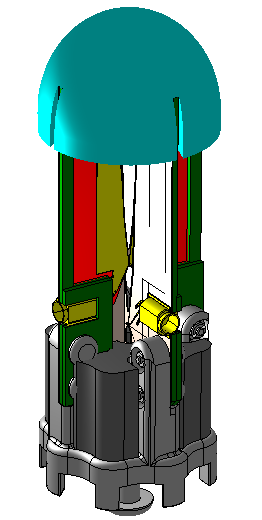
\includegraphics[height=6cm]{Antennas/Vivaldi.png}}
  \centering
  \subfigure[Pattern]{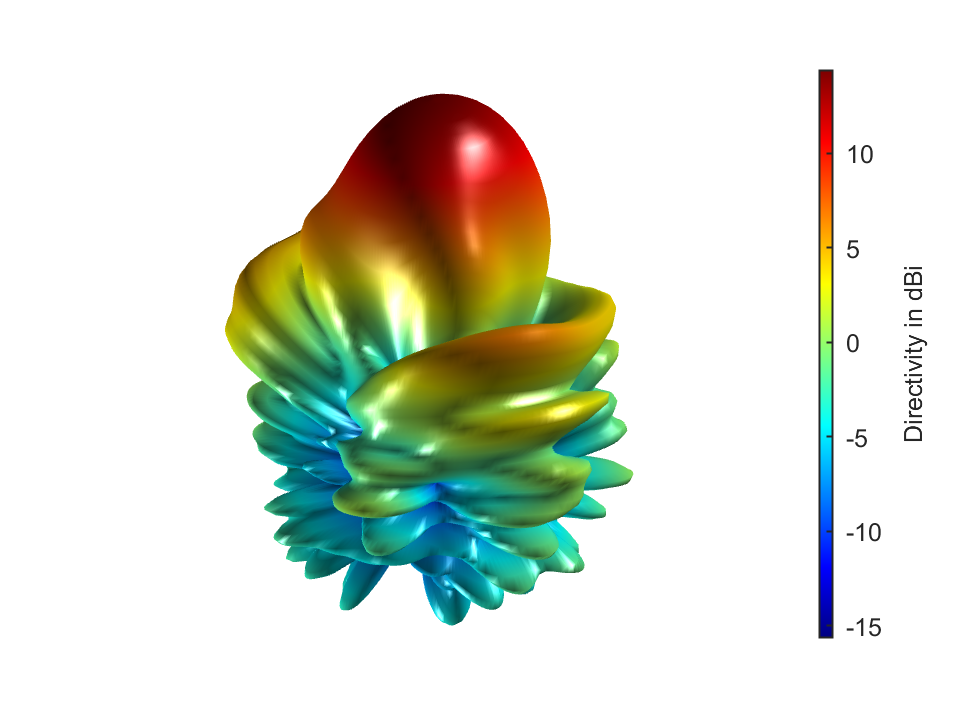
\includegraphics[height=6cm]{Antennas/vivaldi_3D.png}}
\caption{R\&{}S Vivladi TC-TA85CP}
\label{fig:vivpro}
\end{figure}

To show the effects of the different field region high directivity/aperture antennas are used as \ac{DUT}; as probe also low directivity antennas are used. \ac{DUT} antennas:

\begin{itemize}
\item $\SI{20}{\decibel}$ \ac{SGH} LB-28-20 by A-Info depicted in figure \ref{fig:hornpro}.
\item Array of 2x2 $\SI{20}{\decibel}$ \acp{SGH} with $\SI{27}{\decibeli}$ directivity; the pattern is depicted in figure \ref{fig:othera} (b).
\item 10x1 Patch Array from \cite{7481205}, depicted in figure \ref{fig:10x1a} with $\SI{16}{\decibeli}$ directivity
\end{itemize}

Probe antennas:

\begin{itemize}
\item Hertz dipole with $\SI{1.76}{\decibeli}$ Directivity; Pattern in figure \ref{fig:othera} (d).
\item $\sfrac{\lambda}{2}$-dipole with $\SI{2.15}{\decibeli}$ Directivity; Pattern in figure \ref{fig:othera} (c).
\item R\&{}S experimental patch antenna with $\SI{4}{\decibeli}$ directivity depicted in figure \ref{fig:patchpro}.
\item \ac{OEWG} with $\SI{6}{\decibeli}$ directivity depicted in figure \ref{fig:oewgpro}.
\item \ac{RS} Vivladi TC-TA85CP with $\SI{14}{\decibeli}$ directivity depicted in figure \ref{fig:vivpro}.
\item $\SI{20}{\decibel}$ \ac{SGH} LB-28-20 by A-Info depicted in figure \ref{fig:hornpro}.
\item $\SI{26}{\decibel}$ horn depicted in figure \ref{fig:othera} (a).
\end{itemize}

All physical existing antennas are depicted with there simulation model on the left (a) and their directivity pattern on the right (b). Other impractical antennas such as the $\SI{26}{\decibel}$ horn, simulated by a big waveguide port, the 2x2 $\SI{20}{\decibel}$ \ac{SGH} array, the $\sfrac{\lambda}{2}$-dipole, which is at \ac{mmW} wavelength not realisable, and the Hertz-dipole are only depicted with there pattern in figure \ref{fig:othera}.\\
The \ac{RS} Vivladi TC-TA85CP is the standard probe antenna at \ac{RS} with a frequency range from $\SI{4}{\giga\hertz}$ to $\SI{87}{\giga\hertz}$, a gain between $\SI{10}{\decibel}$ and $\SI{20}{\decibel}$ and especially the possibility of measuring both polarisations at the same time with a cross-polarization rejection of greater $\SI{20}{\decibel}$. (figure \ref{fig:vivpro})\\
The $\SI{20}{\decibel}$ \ac{SGH} LB-28-20 by A-Info is normally used to calibrate the measurement setup. It is well known with a lot of empirical data. The underlying WR28-waveguide allows a frequency range from $\SI{26.5}{\giga\hertz}$ to $\SI{40}{\giga\hertz}$. A patch antenna is currently in development at \ac{RS}, it is also used for this simulation and measurement. It is currently not published, so  no further details will be given in this document, except that it has a directivity of $\SI{5}{\decibeli}$, a realized gain of $\SI{3.5}{\decibel}$ and the pattern depicted in figure \ref{fig:patchpro}. 

\subsection{Result of the Range Length Simulation}

The simulation results for all three tested \acp{DUT} is plotted in figure \ref{fig:simres}. In (a), (c) and (e) the \ac{TMP} is plotted over the measurement distance and in (b), (d) and (f) the \ac{EIRP} in the main lobe of the \ac{DUT} is plotted over the measurement distance. It is shown, that the \ac{TRP} measurement error is probe- and range length dependent. The tendency is that, at the same distance the \ac{TMP} error of low directivity probes, such as dipole, patch and \ac{OEWG} is lower than the \ac{TMP} error of high directivity probes, such as Vivaldi and \ac{SGH}. Some similarities between the \ac{TMP} measurement of the \ac{SGH} and the patch array can be found in the course of the graphs. Concluding the \ac{TMP} error is with low directivity probing always lower then $\SI{0.5}{\decibel}$ for greater distances as Derat distance. The individual graph, as well as for the \ac{TMP} and for the \ac{EIRP} in the main lobe, is dependent of the combination of \ac{DUT} and probe. The coarse graph shape of the probe-less simulation from figure \ref{fig:beamcpmp} (c) is recognisable in this complete simulation in figure \ref{fig:simres}.\\
Dynamic range can be increased and measurement effort can be decreased by occupying low directivity probing e.q. with a \ac{OEWG}. For example choosing a \ac{OEWG} instead of the Vivaldi as probe for the \ac{SGH} \ac{TRP} measurement simulation from figure \ref{fig:simres} reduces the the range length for $\SI{0.1}{\decibel}$ measurement error from $\SI{120}{\centi\meter}$ to $\SI{22}{\centi\meter}$ resulting in 

\begin{align*}
G &= \text{FSPL}_{\text{Vivaldi},\SI{0.1}{\decibel}}-\text{FSPL}_{\text{OEWG},\SI{0.1}{\decibel}}+G_\text{OEWG}-G_\text{Vivaldi} \\
G &= \SI{61.4}{\decibel}-\SI{49.3}{\decibel}+\SI{6}{\decibel}-\SI{14}{\decibel} = \SI{6.7}{\decibel}
\end{align*}

%G &= \SI{61.4}{\decibel}-\SI{49.3}{\decibel}+\SI{6}{\decibel}-\SI{14}{\decibel}=\SI{6.7}{\decibel}
%\end{align*}

gain in dynamic range.

\begin{figure}[H]
  \centering
  \subfigure[TMP; DUT: $\SI{20}{\decibel}$ SGH]{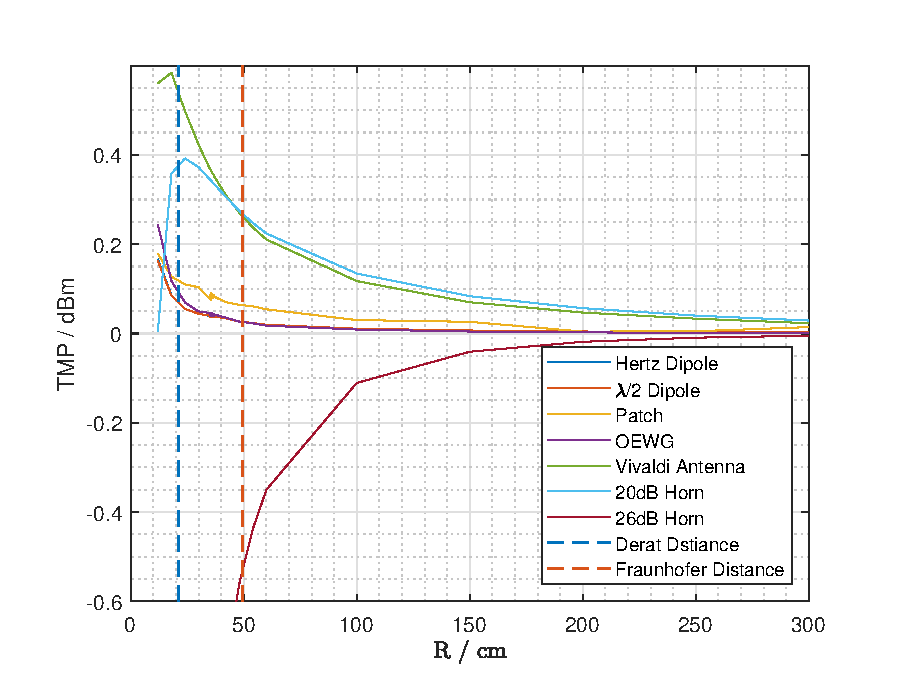
\includegraphics[width=0.49\textwidth]{Matlab/trpDistVivTMP.eps}}
  \centering
  \subfigure[Main EIRP; DUT: $\SI{20}{\decibel}$ SGH]{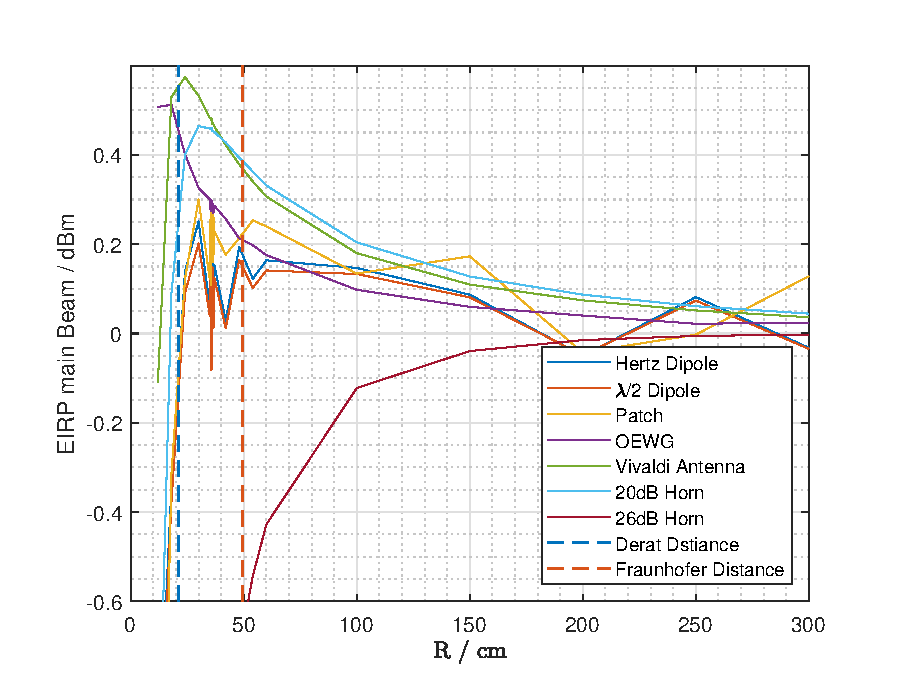
\includegraphics[width=0.49\textwidth]{{Matlab/trpDistVivEIRP.eps}}}
  \centering
  \subfigure[TMP; DUT: 10x1 patch array \cite{7481205}]{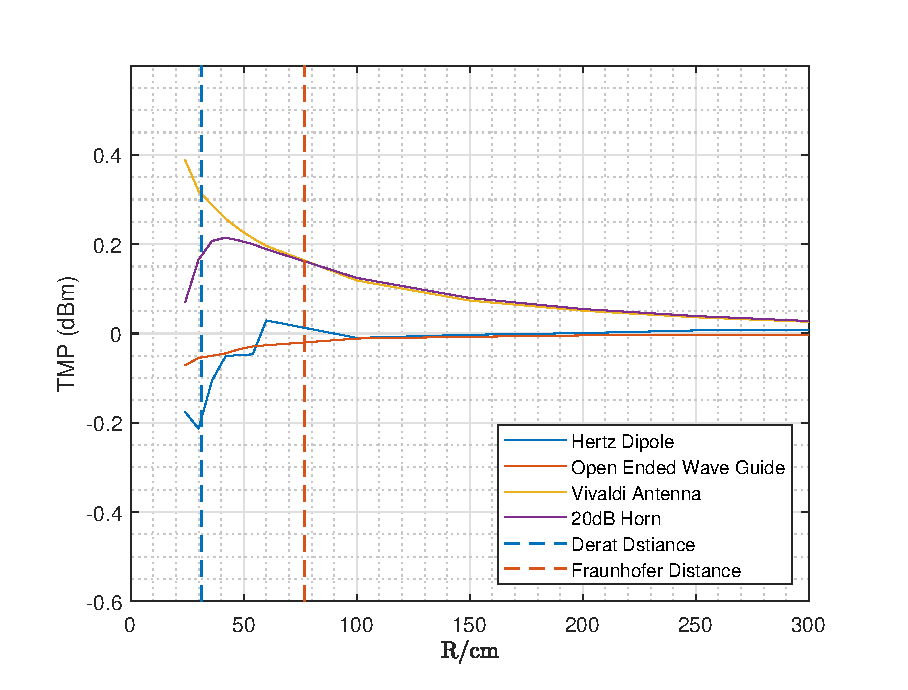
\includegraphics[width=0.49\textwidth]{Matlab/trpDistPaATMP.eps}}
  \centering
  \subfigure[Main EIRP; DUT: 10x1 patch array \cite{7481205}]{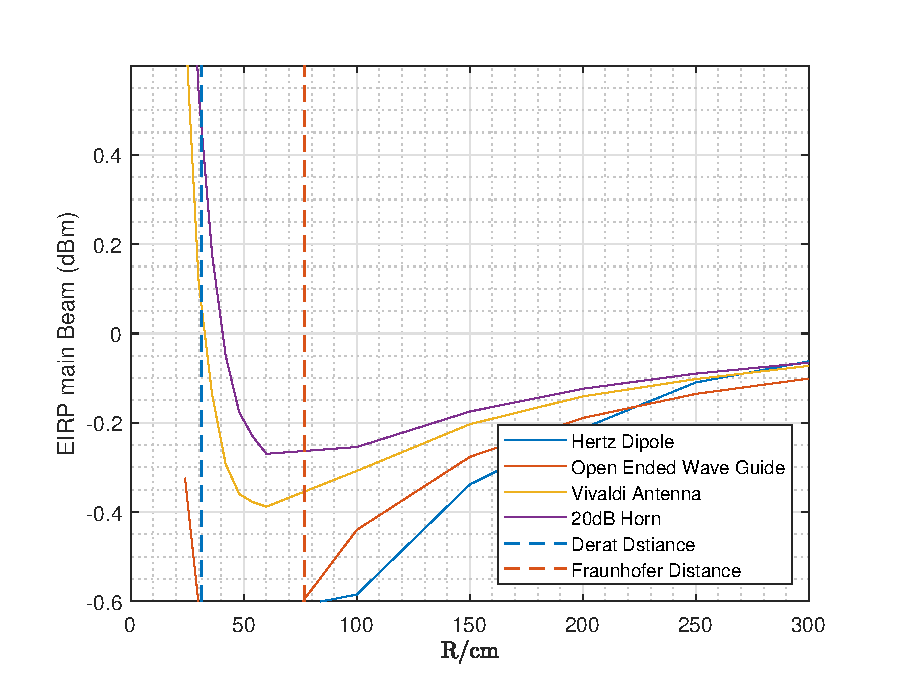
\includegraphics[width=0.49\textwidth]{{Matlab/trpDistPaAEIRP.eps}}}
  \centering
  \subfigure[TMP; 2x2 $\SI{20}{\decibel}$ SGH Array]{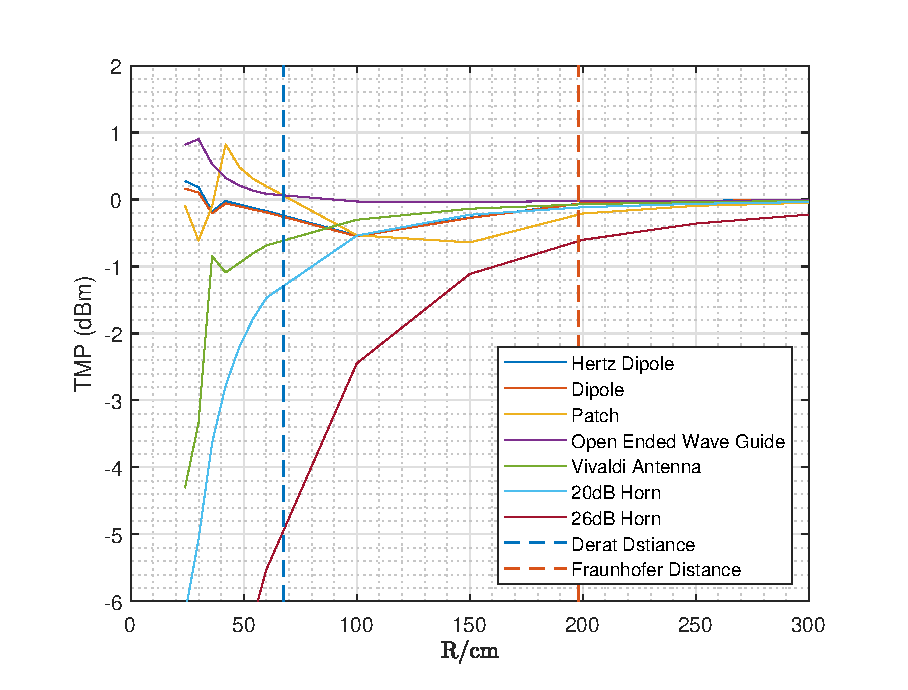
\includegraphics[width=0.49\textwidth]{Matlab/trpDistH2TMP.eps}}
  \centering
  \subfigure[Main EIRP; 2x2 $\SI{20}{\decibel}$ SGH Array]{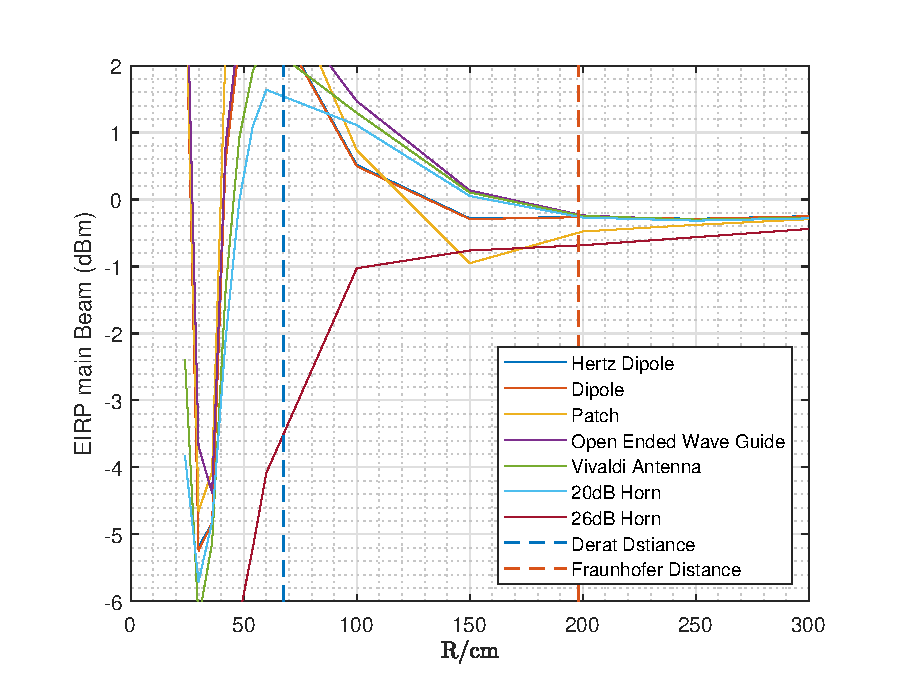
\includegraphics[width=0.49\textwidth]{{Matlab/trpDistH2EIRP.eps}}}
\caption{Simulation results}
\label{fig:simres}
\end{figure}

\section{Measurement to Confirm Simulation Result}

\begin{figure}[H]
\centering
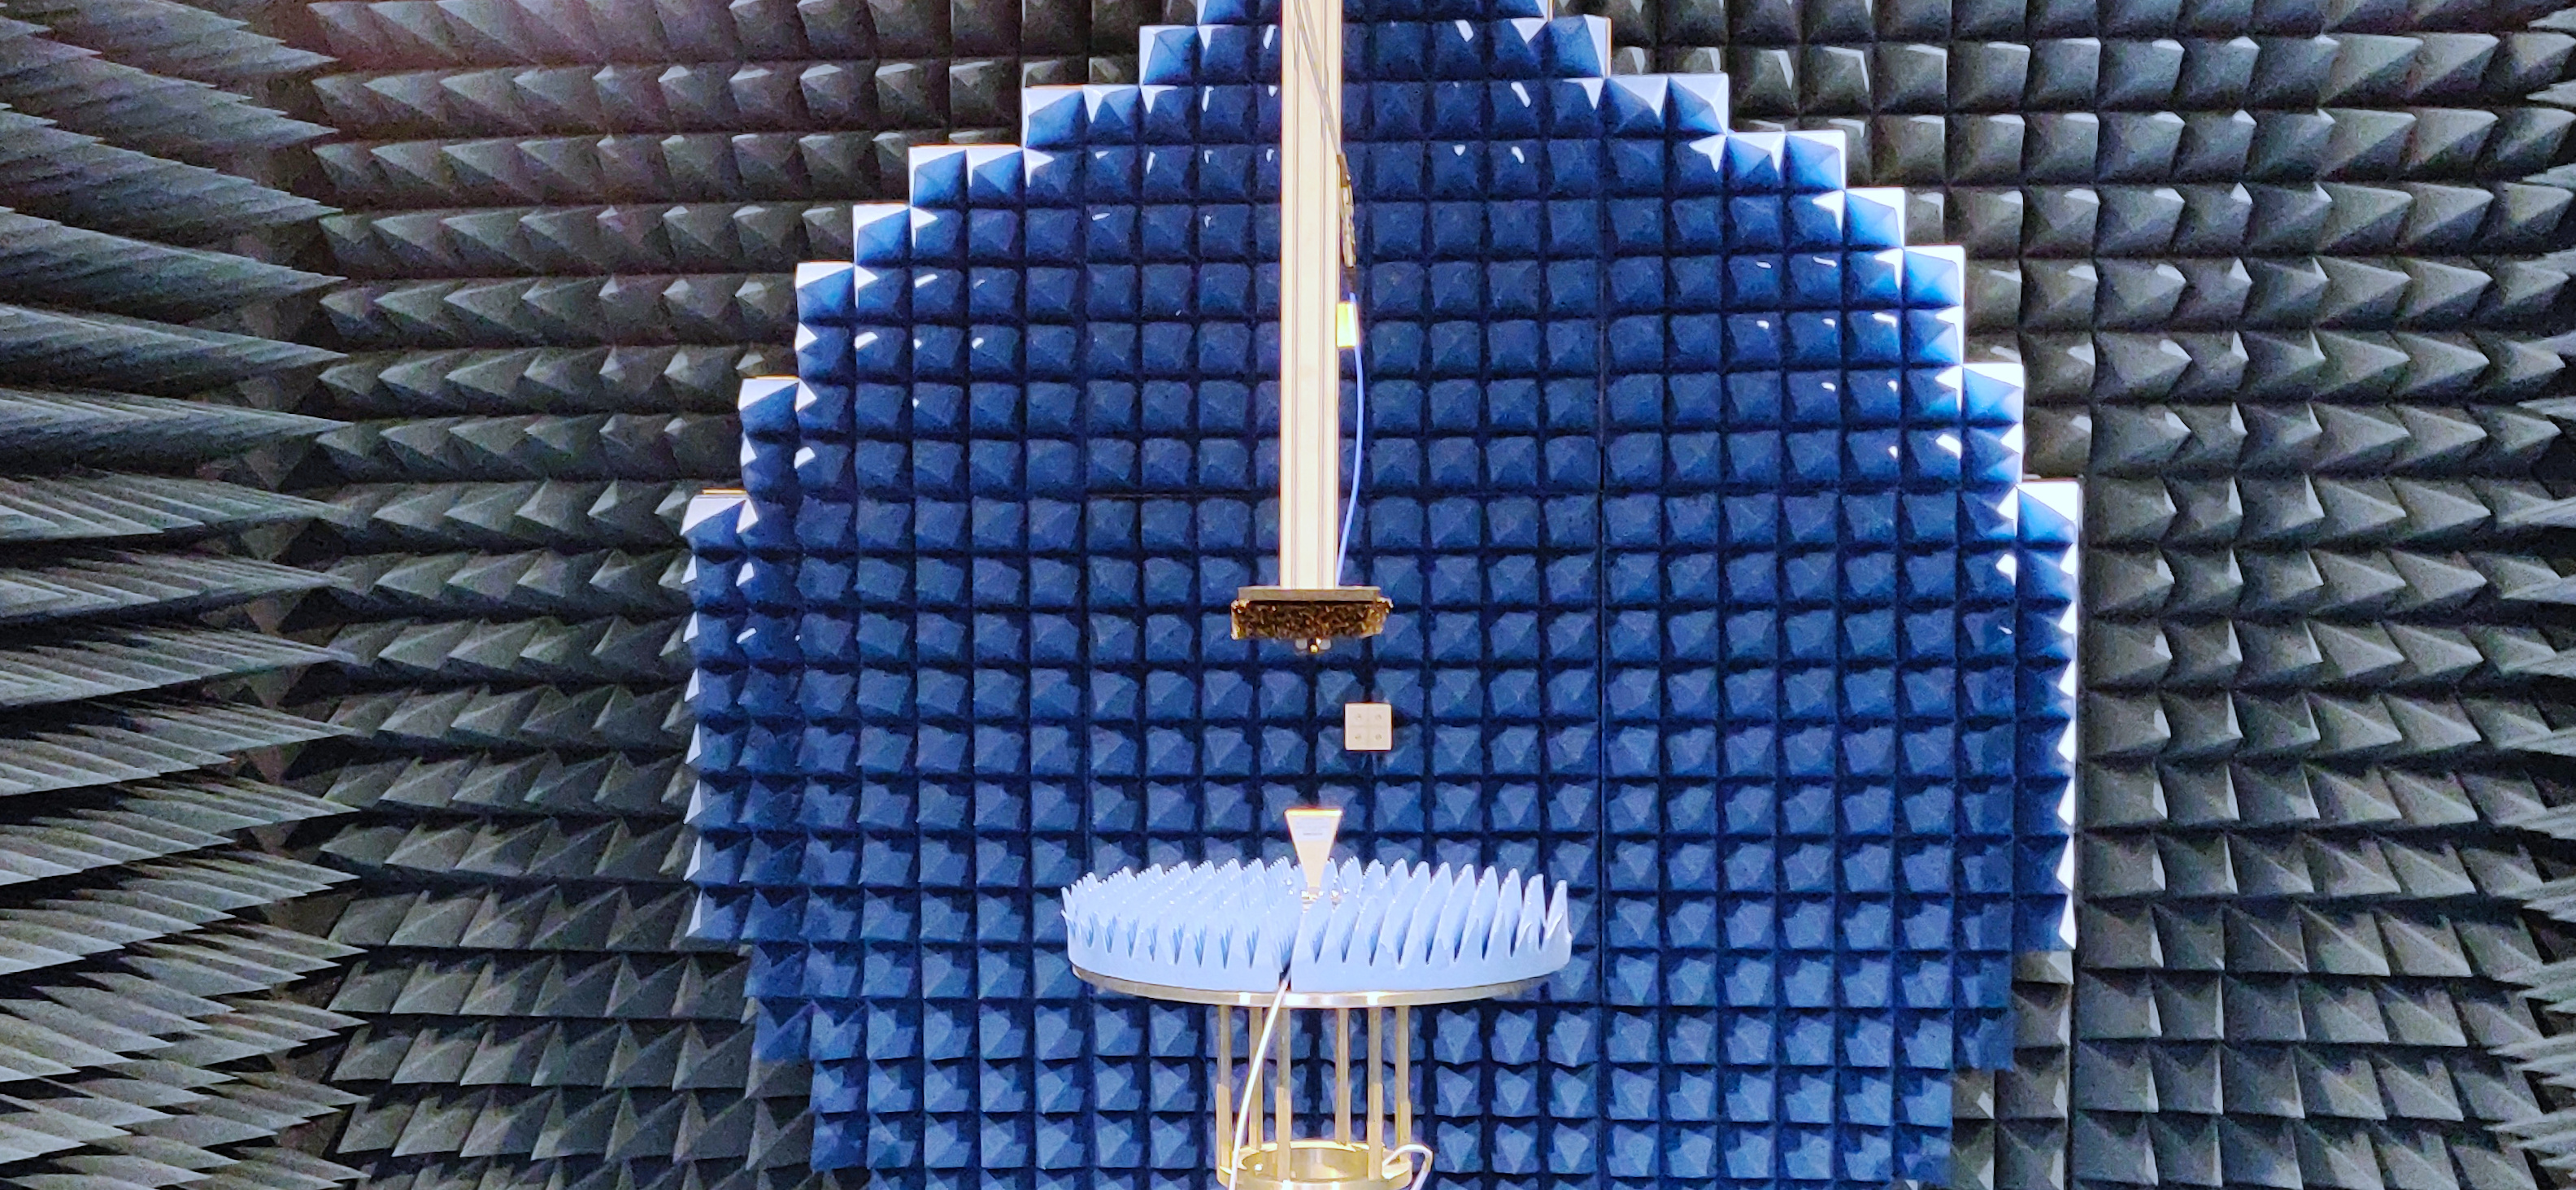
\includegraphics[width=0.8\textwidth]{big-chamber.jpeg}
\caption{OTA Measurement for minimum rangelength measurement series; DUT: $\SI{20}{\decibel}$ SGH; probe: Patch}
\label{fig:otameas}
\end{figure}

To proof the introduced simulation to investigating \ac{NF} probing for \ac{TRP} measurements this test is done in a \ac{WPTC} depicted in figure \ref{fig:otameas}, located in the \ac{RS} headquarters in Munich using a \ac{RS} \ac{VNA} 67.

\subsection{Implementation}

 Because of the high cable loss resulting from long cables caused by the big chamber a $\SI{40}{\decibel}$ azimuth amplifier is used. Only the A-Info $\SI{20}{\decibel}$ \ac{SGH} was used as \ac{DUT} on the azimuth table with it's aperture in the center of rotation. This adds an other $\SI{3}{\centi\meter}$ radius to the phase center. Occupying a low gain probe such as the Patch, the maximum range length of about $\SI{1.1}{\meter}$ and a \ac{RBW} of $\SI{100}{\hertz}$ results in a dynamic range of about $\SI{20}{\decibel}$. This is not pleasant to plot the pattern, but it's sufficient to compute an adequate \ac{TMP}. To adjust the radius a aluminium profile is used, refer to figure \ref{fig:otameas}. Because of the mounting on the azimuth turn table, the elevation can only be measured from $\theta_\text{min}=\SI{0}{\degree}$ and $\theta_\text{max}=\SI{85}{\degree}$. This is sufficient regarding the \ac{SGH}s pattern in figure \ref{fig:hornpro}. As in the simulation a $\SI{5}{\degree}$-\ac{CSSG} is used with swept azimuth and therefore hardware triggering from the positioner to the \ac{VNA}. So that one \ac{TRP} measurement takes around $\SI{2}{\min}$.

\subsection{Set Up}

\begin{figure}[H]
  \centering
  \subfigure[WR28 OEWG 1]{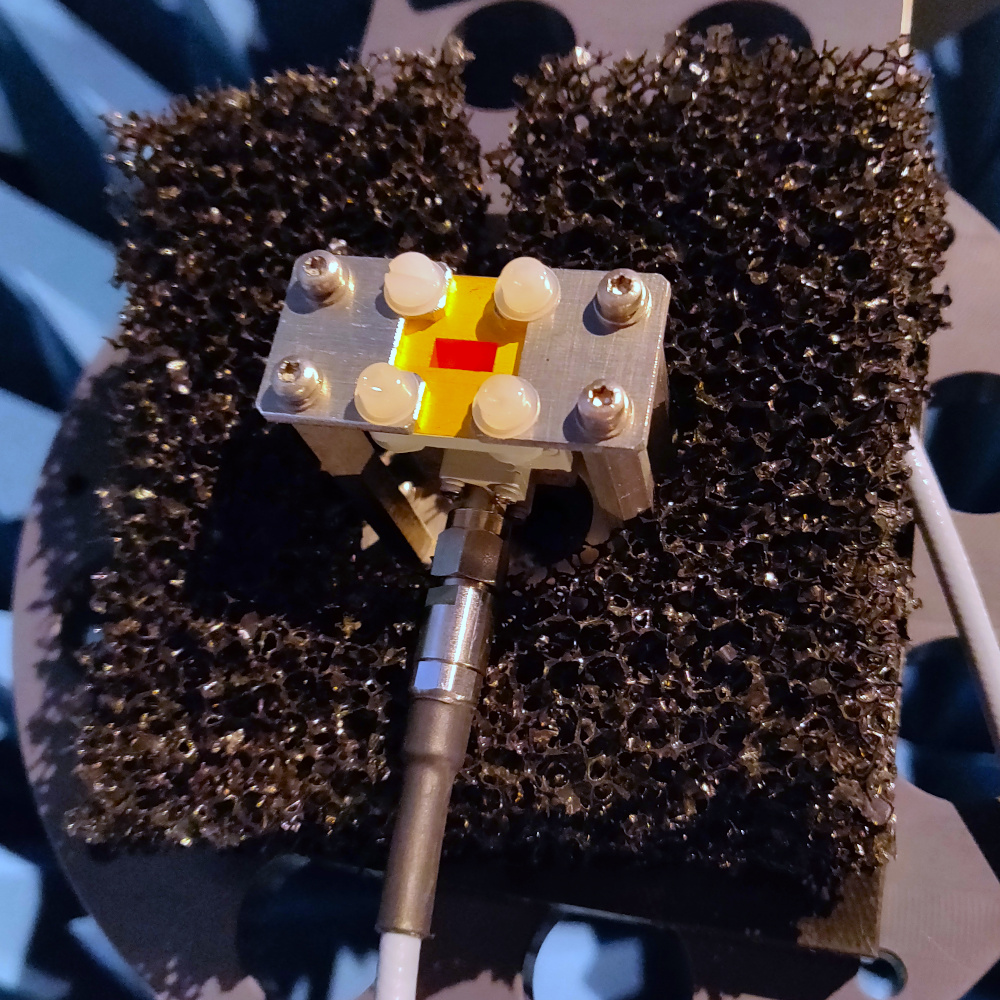
\includegraphics[width=0.3\textwidth]{OEWG-Imp1.jpg}}
  \centering
  \subfigure[WR28 OEWG 2]{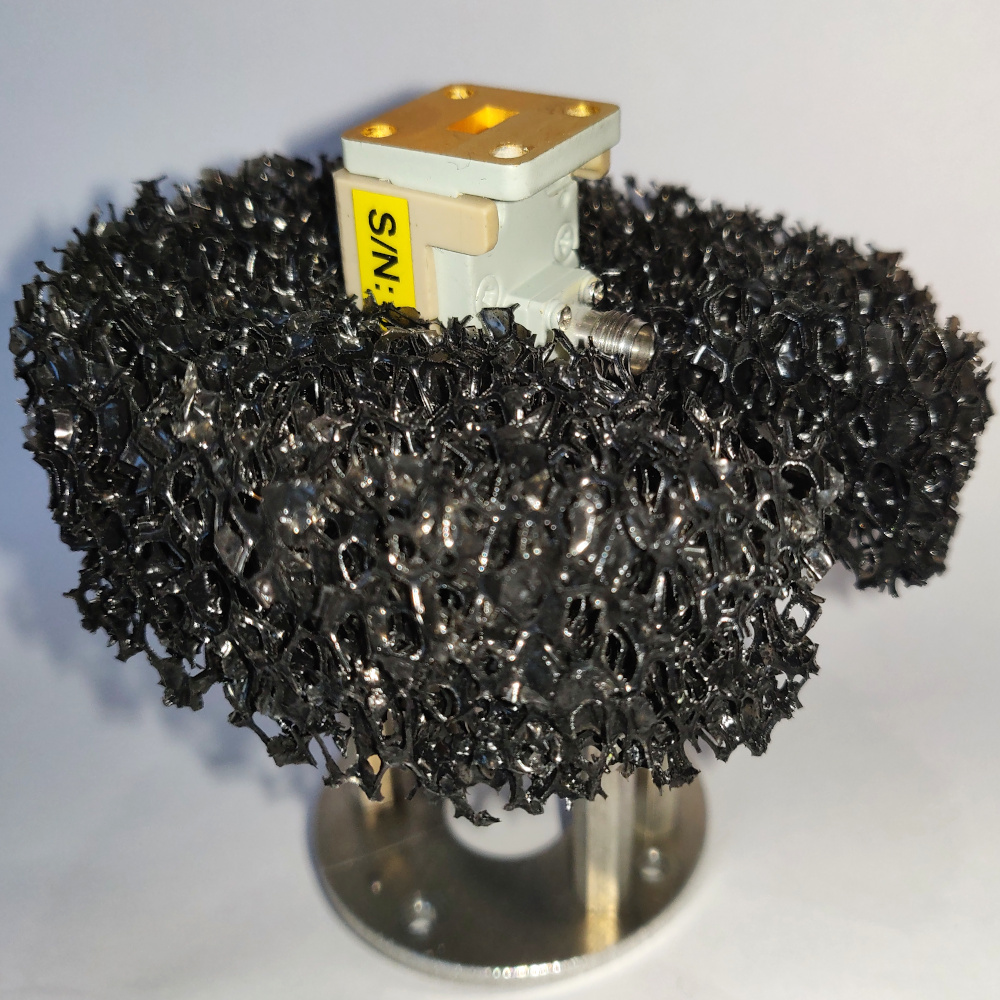
\includegraphics[width=0.3\textwidth]{OEWG.jpg}}
  \centering
  \subfigure[Mounted Patch antenna]{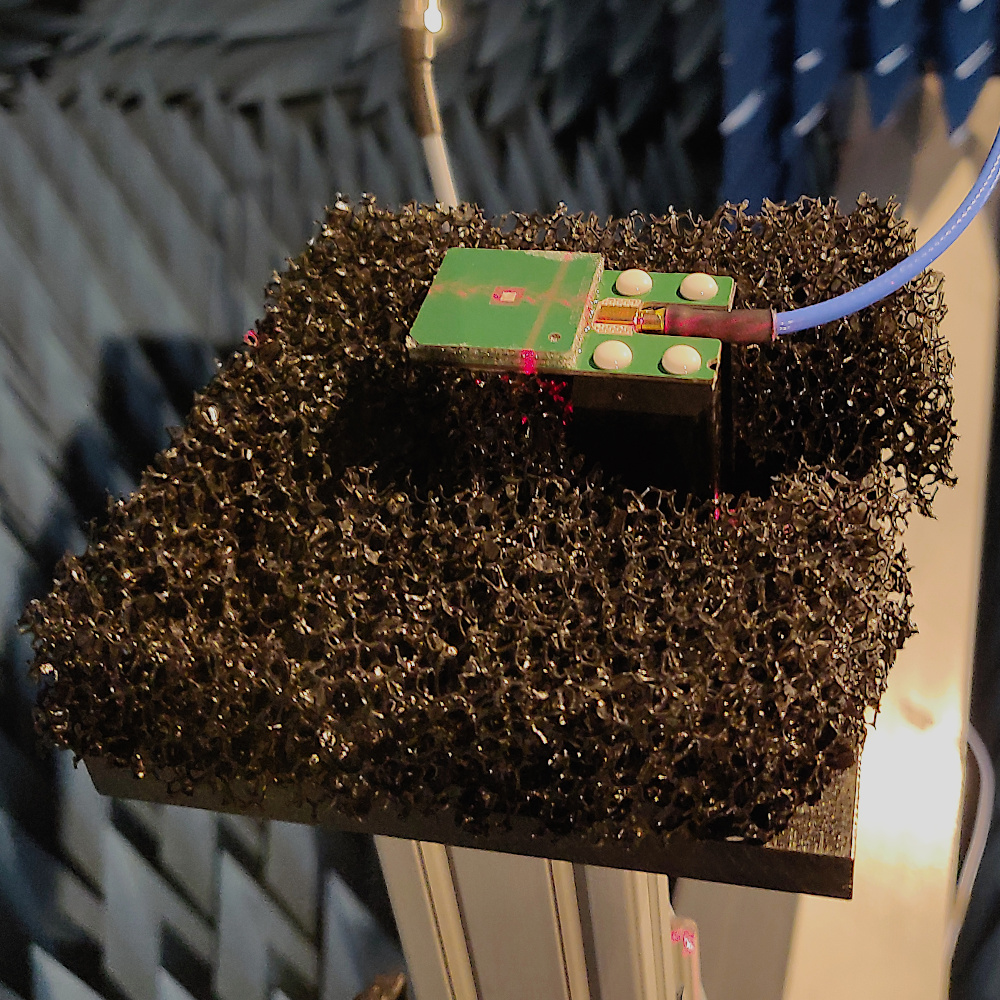
\includegraphics[width=0.3\textwidth]{Patch.jpg}}
\caption{Real implementation of probe antennas}
\label{fig:realprobe}
\end{figure}

The minimum and maximal measurement sphere radius varies because of the probe mounting from around $\SI{10}{\centi\meter}$ to around $\SI{115}{\centi\meter}$. From $\SI{10}{\centi\meter}$ to $\SI{16}{\centi\meter}$, $\SI{1}{\centi\meter}$ radius increment, from $\SI{16}{\centi\meter}$ to $\SI{20}{\centi\meter}$ $\SI{2}{\centi\meter}$ radius increment and than $\SI{5}{\centi\meter}$ radius increment is occupied. The measurement is carried out by using the $\SI{20}{\decibel}$ \ac{SGH} LB-28-20 by A-Info (figure \ref{fig:hornpro}), the Vivaldi (figure \ref{fig:vivpro}), the Patch (figure \ref{fig:realprobe} (c)) and the two \ac{OEWG} implementations (figure \ref{fig:realprobe} (a) and (b)) as probe and the $\SI{20}{\decibel}$ \ac{SGH} as \ac{DUT}. There are some issues with the probe implementations depicted in figure \ref{fig:realprobe}:

\begin{enumerate}[label=(\alph*)]
\item Because no WR28 \ac{OEWG} antenna was available, a WR28 wave guide adapter and a \ac{SGH} mounting was first taken. With the metal in front of the aperture the \ac{FF} pattern differs from a real \ac{OEWG} and the directivity increases by around $\SI{4}{\decibel}$. This was simulated in CST\texttrademark{} and the resulting antenna pattern is plotted in figure \ref{fig:oewgimpone}.
\item With an other mounting the aperture is free from additional metal. The problem is here, that the metal plate surrounding the opening of the wave guide reflects the \ac{EM} waves emitted to it. This leads to standing waves in the \ac{NF}.
\item The patch is a omnidirectional radiator (refer to figure \ref{fig:patchpro}). With the absorbers, the directivity of this antenna is rising, because the \ac{TRP} is diminishing by absorbing the backwards orientated radiation. Additionally the patch antenna is placed on a ground plane, which leads similar to the wave guide adapter from (b) to standing waves and \ac{EM} scattering back to the source.
\end{enumerate}

\subsection{Result}

\begin{figure}[H]
  \centering
  \subfigure[TMP over measurement distance]{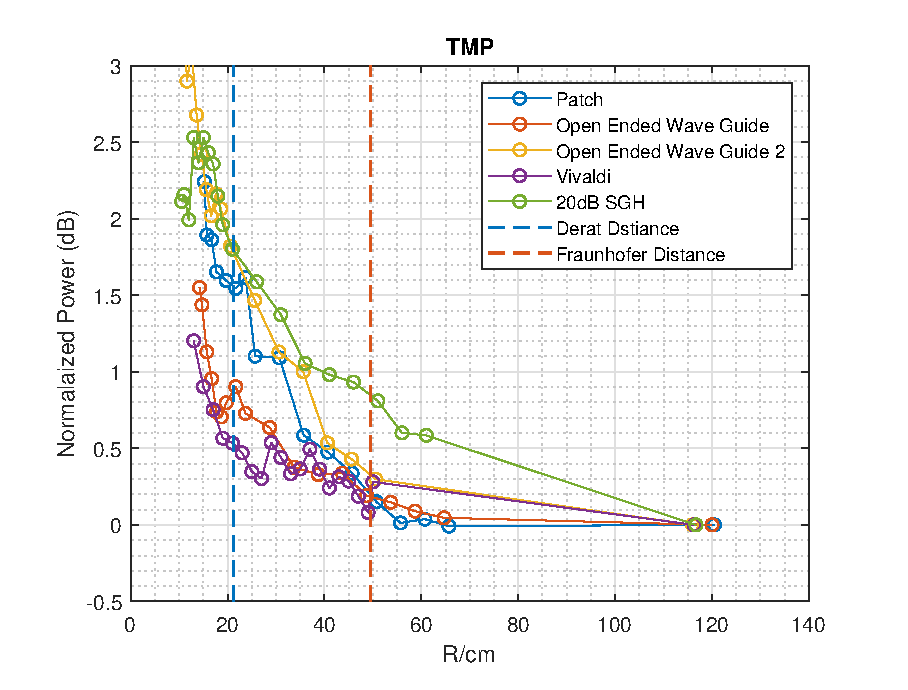
\includegraphics[width=0.49\textwidth]{Matlab/measSGHTMP.eps}}
  \centering
  \subfigure[Main EIRP over measurement distance]{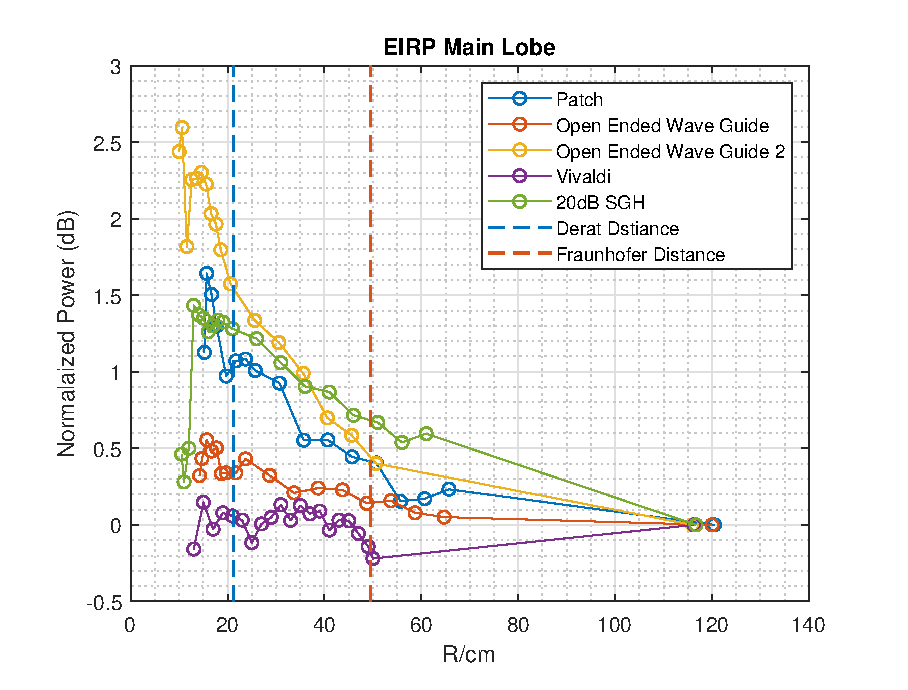
\includegraphics[width=0.49\textwidth]{{Matlab/measSGHEIRP.eps}}}
\caption{Measurement result: DUT $\SI{20}{\decibel}$ SGH}
\label{fig:meastrpdistviv}
\end{figure}

Leaving the \ac{OEWG} and the patch antenna the tendency that lower directivity probes grant less \ac{TRP} error at the same measurement distance is proved regarding the graph from $\SI{20}{\decibel}$ \ac{SGH} and Vivaldi in figure \ref{fig:meastrpdistviv} (a). Also the \ac{EIRP} in the main lobe measured by the \ac{SGH} has similar characteristics than the simulation. The \ac{OEWG}-implementation one has a similar \ac{TMP} characteristic as the Vivaldi. This is caused by the $\SI{4}{\decibel}$ higher gain induced by the mounting. Both, the \ac{OEWG} two and the patch, have similar characteristics in terms of \ac{TMP} and main \ac{EIRP} caused by the, in the previous section described scattering of the grounded planes.\\
In the simulation it is assumed that the characteristics and behaviour of the \ac{DUT} is independent from the probe, thus the vector-EM-field in the volume is independent from the used sampling probe. This is a valid assumption for \ac{FF} or for probes with little scattering back to the \ac{DUT}. 
The Vivaldi probe shows similar simulation and measurement results figure \ref{fig:simres} (a) and figure \ref{fig:meastrpdistviv} (a). Bigger impact is recognized comparing the graph of the \ac{SGH} probe simulation to the measurement. 
There are two main reasons for that. First this can be caused by the greater amount of metal and the physical shape of it, put in the \ac{NF}-volume of the \ac{DUT}.
It is shown in figure \ref{fig:meastrpdistviv} (a), that the \ac{OEWG}2 and the patch are having less \ac{TMP}-error in the \ac{FF} of the \ac{DUT}. In the \ac{DUT}s \ac{NF} the measurement result is sharply rising till it is similar with the $\SI{16}{\decibel}$ more directive \ac{SGH}. This is caused by the change of the \ac{EM} vectorfield from the \ac{DUT} induced by the probe. This phenomena is also visible plotting the \ac{EIRP}-pattern of the \ac{SGH} \ac{DUT} in different measurement radii. Comparing the measured antenna pattern from the Vivaldi probe (figure \ref{fig:sghpatternvivaldi}) to the \ac{OEWG}2 (figure \ref{fig:sghpatternoewg2}) and the patch (figure \ref{fig:sghpatternpatch}) shows additionally to the evolving pattern over distance (compare figure \ref{fig:devantennap}) some fluctuations in the surrounding of the main lobe. The center of rotation is chosen to be the center of the aperture $\SI{3}{\centi\meter}$ away from the phase center of the horn, leading to fine range length differences and thereby to different standing wave modes explaining the fluctuation. This fluctuation is not visible in the pattern of the Vivaldi probe from fig. \ref{fig:sghpatternvivaldi}.\\
Second the power acceptance of the probe antennas could not be simulated. So additional to the physical shape of the antenna, the power reflected from the probe antenna causes additional interference at the \ac{DUT}. Because of the low directivity of the \ac{OEWG} or the patch this effect should be less impactful than the general scattering.

\section{Conclusion}

The simulation showed that low directivity probes such as the \ac{OEWG} can be used to measure the \ac{TRP} at lower distances compared to high directivity probes such as the Vivaldi antenna. The tendency is proofed by the measurement. The \ac{OEWG} measurement must be repeated due to the reasons discussed in the section above.





